\documentclass[a4paper, 15pt]{article}
\usepackage[left=0.85in, right=0.85in, top=0.5in, bottom=0.95in]{geometry}
\usepackage[T1]{fontenc}
\usepackage[utf8]{inputenc}
\usepackage[italian]{babel}

% Formattazione del testo
\usepackage{setspace}         % Setting dello spazio\begin{spacing}{0.95}
\setstretch{1.2}
\setlength{\parindent}{0pt}
\raggedbottom
\usepackage[none]{hyphenat}    % no sillabazione 
\usepackage{multicol}          % testo su più colonne
\usepackage{changepage}	       % \begin{adjustwidth}{}{}

% Matematica
\usepackage{amsmath, amssymb, amsthm, mathtools}
\usepackage{cancel}            % semplificazioni \cancel{expression}
\newtheorem*{thm}{Teorema}
\newtheorem*{en}{Enunciato}
\newtheorem*{definizione}{Definizione}
\newtheorem*{cor}{Corollario}
\DeclareMathOperator{\rk}{rk}
\DeclareMathOperator{\im}{Im}
\DeclareMathOperator{\ev}{ev}

% Simboli e Disegni
\usepackage{color}             % \textcolor{'ColorCode'}{'testo'}
\usepackage{graphicx, wrapfig, float}
\usepackage{fancyhdr}
\usepackage{tikz, circuitikz}
\usepackage{tkz-euclide}
\usetikzlibrary{patterns, arrows, decorations.markings, arrows.meta, decorations.text}
\tikzset{immagine/.style={above right, inner sep=0pt, outer sep=0pt},
	testo/.style={fill=white, align=center, fill opacity=0.6, text opacity=1, below, font=\sffamily\bfseries\footnotesize}}
\usepackage{pgfplots}
\pgfplotsset{compat=1.15}
\usepackage{mathrsfs}

% Altri pacchetti
\usepackage{enumitem}
\usepackage{mdwlist} 	       % suspend enumerate \suspend{} \resume{}
\usepackage{siunitx}
\usepackage{hyperref}
\hypersetup{
	colorlinks=true,
	linkcolor=blue,    
	urlcolor=blue,
}
\urlstyle{same}

% Altre definizioni personali
\usepackage{pifont}
\newcommand{\cmark}{\ding{51}}
\newcommand{\xmark}{\ding{55}}
\DeclareUnicodeCharacter{20AC}{\EUR}
\newcommand{\compresslist}{\setlength{\itemsep}{1pt}\setlength{\parskip}{0pt}\setlength{\parsep}{0pt}}
\newcommand{\ra}[1]{\renewcommand{\arraystretch}{#1}} % stretcho le tabelle e gli array \ra{x}
\setlength{\jot}{10pt}

%=======HEADER & FOOTER=======%
\def\lesson{Lezione N.26}


\pagestyle{fancy}
\fancyhf{}
\renewcommand{\headrulewidth}{0pt}
\renewcommand{\footrulewidth}{1.4pt}
\lfoot{A.M. $\diamond$ \the\year}
\cfoot{\thepage}
\rfoot{\lesson}


% Titolo e data
\title{Parte 18: ruote cilindriche corrette}
\date{}
		
		\begin{document}
			\maketitle
			\setcounterpageref{secnumdepth}{0}
			\setcounter{tocdepth}{5}  % Includo nel TOC anche i subsubpar	
			\tableofcontents 
			\newpage
			
			
			
			%\end{adjustwidth}
			%\newpage
			\section{Dentature ad evolvente corrette}
			\begin{adjustwidth}{2in}{}	
				Si è visto che la riduzione dei massimi degli strisciamenti specifici possono essere ridotti riducendo il segmento dei contatti attraverso il taglio con interferenza della ruota. 
				
				Questa tecnica tuttavia non permette di bilanciare questi strisciamenti, a tal fine, e anche per andare incontro ad esigenze di compattezza della trasmissione - e quindi di riduzione di interasse tra ruota e pignone,  si utilizza una tecnica di taglio chiamata \textbf{correzione dell'evolvente}. 
				
				Questa tecnica si può utilizzare esclusivamente in presenza di taglio indiretto, cioè mediante inviluppo. \newline 
				
				Per realizzare il dimensionamento di una ruota dentata si deve partire da un proporzionamento modulare, ovvero scegliere un valore standard di modulo tra quelli riportati in tabella.
				\begin{figure}[H]
					\centering
					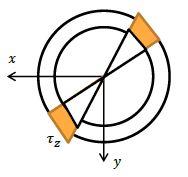
\includegraphics[width=0.5\linewidth]{figures/screenshot001}
					\caption{I valori tra parentesi sono SCONSIGLIATI}
					\label{fig:screenshot001}
				\end{figure}
				Sono espressi in mm e danno un'indicazione della proporzione, maggiore è il modulo e maggiore sarà la robustezza e la resistenza del dente. Naturalmente, maggiore sarà il modulo, a parità di numero di denti, si avranno maggiori dimensioni della ruota. \newline
				
				Per ridurre le dimensioni della trasmissione, una volta fissato il modulo per motivi di resistenza, si deve per forza ridurre il numero di denti. 
				
				Al di sotto di un certo numero di denti ci si imbatte tuttavia nell'interferenza di funzionamento e scavando troppo il dente, lo si indebolisce.
				
				Come si può allora ridurre le dimensione dell'ingranaggio? Attraverso la correzione. 
				
				Si realizza un taglio per inviluppo a cerchi spostati. 
				\begin{figure}[H]
					\centering
					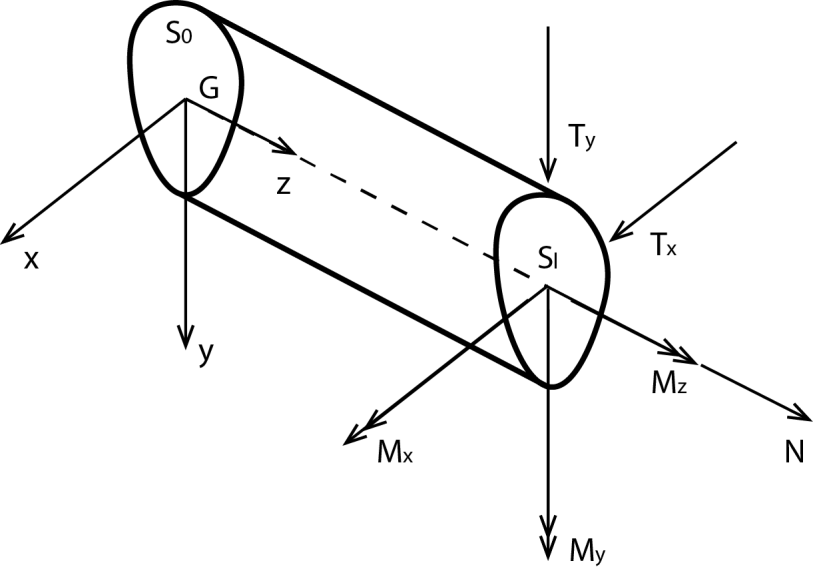
\includegraphics[width=0.7\linewidth]{figures/screenshot002}
					\label{fig:screenshot002}
				\end{figure}
				
				In pratica quando avviene l'accoppiamento dentiera-rocchetto si accoppiano due entità cinematiche: la circonferenza primitiva del rocchetto e una retta di riferimento della dentiera, a quel punto la dentiera durante il funzionamento lascia un'impronta sul rocchetto e scava i denti del rocchetto. 
				
				ma se si immagina di traslare la dentiera reale rispetto alla retta di riferimento, l'importa lasciata  sarà diversa, la rulletta dell'apice del dente, in dipendenza della posizione in cui viene posto - lasciando inalterate detta di riferimento e primitiva -  lascia una diversa impronta. 
				
				L'altezza del dente ovviamente non cambia, ciò che si modifica è la sporgenza della dentiera rispetto alla retta di riferimento: la correzione non è altro che la variazione  dei parametri cinematici del moto tra dentiera e rocchetto. 
				
				La circonferenza del rocchetto rispetto alla quale si verifica l'accoppiamento si chiamerà \textbf{primitiva di taglio, di lavorazione}  e questa sarà tangente ad una retta di riferimento spostata di una certa quantità $x\cdot m_0$. 
				
				Si indicheranno d'ora in poi con lo "0" al pedice tutte quelle grandezza riferite alla fase di taglio: $m_0$ è il modulo della dentiera. 
				
				Ricordando sempre che dalla figura sopra, quell'altezza $h = {m\over}$ contribuirà soltanto a creare il raggio di raccordo al piede. 
				
				Quando la nuova posizione  della retta di riferimento è spostata verso l'apice della dentiera allora è una correzione \textbf{positiva}, se invece la retta di riferimento è spostata verso la base della dentiera, la correzione sarà \textbf{negativa}. 
				
				Questo spostamento determina esclusivamente  una variazione delle grandezza cinematiche di taglio. \newline 
				
				Che risultati si ottengono con la correzione? 
				
				Si ottengono denti dalle forme differenti in funzione del tipo di correzione,  fissato un cerchio primitivo si hanno denti con correzione positiva da una forma larga alla base, robusta ma tendente al dente a punta, una correzione negativi invece porta ad un dente molto assottigliato alla base. 
				\begin{figure}[H]
					\centering
					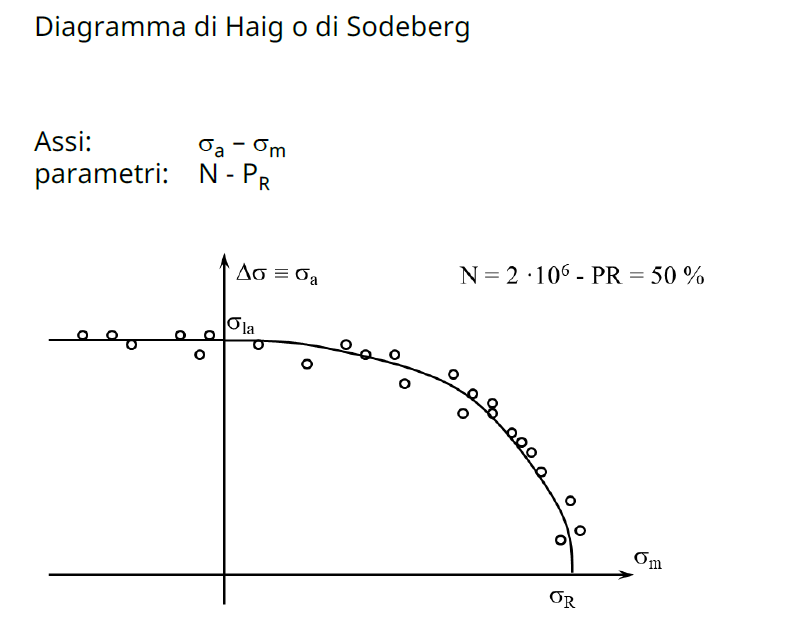
\includegraphics[width=0.5\linewidth]{figures/screenshot003}
					\label{fig:screenshot003}
				\end{figure}				
				La scelta de coefficiente di correzione viene fatta in fase ei realizzazione della ruota, si ottengono potenzialmente infinite  geometrie diverse di ruota dentata utilizzando lo stesso rocchetto e la stessa identica dentiera, questa infatti viene identificata da un modulo $m_0$ e da un angolo $\theta_0$ tra il profilo retto della dentiera e la sua normale, rispetto all'orizzontale, che viene detto \textbf{angolo di attacco}, che per correzione nulla è esattamente pari all'angolo di pressione, mentre in presenza di correzione, è proprio della dentiera, mentre l'angolo di pressione potrà in alcuni casi differire. \newline 
				
				Realizzando un accoppiamento ruota-pignone si dovranno scegliere i coefficienti correttivi relativi a pignone e ruota. 
\end{adjustwidth}
%\newpage
\section{Correzioni Lasche}
\begin{adjustwidth}{2in}{}				
				La correzione più semplice è quella teorizzata da Lasche che impone l'applicazione di una correzione $x$ positiva sul pignone  ed una correzione negativa sulla ruota pari esattamente a $x' = -x$, in pratica si sta realizzando un pignone con addendum più sporgente ed una ruota con addendum meno sporgente, proprio ciò che si cercava di fare per ridurre l'interferenza. 
				
				L'altezza del dente - si ripete - rimane inalterata: si spostano le rette di riferimento ma l'utensile che scava è sempre lo stesso. \newline 
				
				Avendo spostato in questo modo i cerchi di riferimento di taglio, sulla primitiva, l'arco che descrive lo spessore del dente, è sostanzialmente cambiato, mentre il passo su ruota e pignone è rimasto identico. 
				\begin{figure}[H]
					\centering
					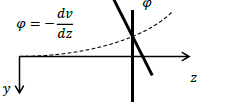
\includegraphics[width=0.5\linewidth]{figures/screenshot004}
					\label{fig:screenshot004}
				\end{figure}
				
				Se senza correzione lo spessore era pari alla metà del passo, ora invece lo spessore sulla primitiva di taglio, sarà diverso sia per ruota che per pignone. 
				\[\begin{dcases}
					s_0' = \dfrac{\pi m_0}{2} + 2x'm_0\tan\theta_0 \underset{Lasche}{=} \dfrac{\pi m_0}{2} - 2xm_0\tan\theta_0 \\
					s_0 = \dfrac{\pi m_0}{2} + 2xm_0\tan\theta_0
				\end{dcases}\]
				\textbf{Queste due relazioni sono valide qualunque sia la correzione}. 
				
				Effettuando la somma dei due spessori per verifica l'ingranamento della ruota dentata, il risultato, per correzioni Lasche, è il seguente
				\[\dfrac{\pi m_0}{2} - \cancel{2xm_0\tan\theta_0} + \dfrac{\pi m_0}{2} + \cancel{2xm_0\tan\theta_0} = \pi m_0 = p\]
				Ovvero esattamente il passo. 
				
				La condizione di ingranamento scritta in termini generici per ruote non corrette - cioè che la somma degli spessori sulle primitive deve essere pari al passo - per correzione Lasche, permette di ingranare le ruote mantenendo INALTERATO l'interasse, ovvero ottimizzando le primitive di taglio come primitive di lavoro: le circonferenze primitive usate nell'intaglio si possono usare anche per l'accoppiamento cinematico ruota-pignone esattamente come si faceva per le ruote non corrette. 
\newpage 				
				Per cui per correzioni Lasche
				\begin{itemize}
					\item rimane invariato il modulo
					\item rimane invariato l'angolo di pressione 
					\item rimane invariato l'interasse
					\item rimane invariata l'altezza dei denti
					\item cambiano soltanto le primitive, di una quantità $xm_0$
				\end{itemize}
				
				L'effetto, dal punto di vista della forma del dente, è già stato discusso. 
				\begin{figure}[H]
					\centering
					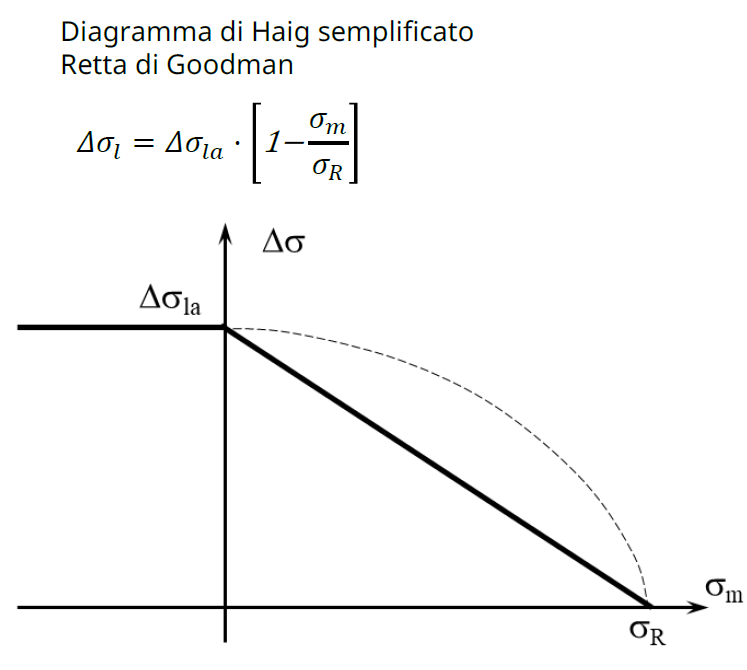
\includegraphics[width=0.5\linewidth]{figures/screenshot005}
					\label{fig:screenshot005}
				\end{figure}
				La tendenza è molto simile all'effetto di un intaglio a diversi angoli di pressione, per $\theta\uparrow$ si otteneva un dente tozzo, mentre se $\theta\downarrow$ un dente fine, la sostanziale differenza sta nel fatto che con una correzione Lasche si ottengono queste forme senza variare nè l'interasse, nè le spinte sull'albero. \newline 
				
				Per una correzione positiva, se aumenta lo spessore alla base, diminuisce quello in testa, e allora il valore dello spessore in testa dovrà essere tenuto sotto controllo. 
				
				Nel seguente grafico si individua la variazione di spessore in testa normalizzato rispetto al modulo. 
				 \begin{figure}[H]
				 	\centering
				 	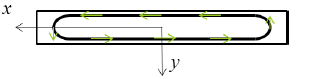
\includegraphics[width=0.7\linewidth]{figures/screenshot006}
				 	\label{fig:screenshot006}
				 \end{figure}
				 Si entra col numero di denti della specifica ruota, si individua la curva col coefficiente di correzione scelto, si legge a questo punto il valore in ordinata dello spessore alla base normalizzato il modulo e ricavando la curva di tendenza si può leggere il valore dello spessore in testa normalizzato il modulo. 
				 
				 Questo diagramma dice che ad una forte riduzione del numero di denti o all'aumento eccessivo della correzione, si ottengono spessori alla base molto elevati ma spessori in testa molto ridotti. 
				 
				 A parità di numero di denti, con correzioni negative, si otterrà il trend opposto. \newline 
				 				 
				 C'è un altro effetto della correzione estremamente importante ed è legato al numero  minimo di denti teorico che garantisce la non interferenza, infatti per essere  tagliati senza interferenza, la relazione era 
				 \[z_0 = \dfrac{2k'}{\sin^2\theta}\]
				 $k'$ era la sporgenza della ruota coniugata al rocchetto, il profilo efficace della dentiera, in condizioni non corrette vale 1 perché rispetto alla retta di riferimento la dentiera sporge di una quantità pari a: 
				 \[{5\over4}m - {1\over4}m\]
				 Per cui la parte effettiva che taglia il dente è pari a $m$. 
				 
				 Nel caso di correzione, e quindi nel caso in cui si sposti questa retta di riferimento, la sporgenza cambia, per cui varrà 
				 \[k' = 1- x \qquad k'= 1-x'\]
				 Di conseguenza cambia il numero minimo di denti intagliabile senza interferenza, questo è un grandissimo vantaggio perché per correzioni positive si ottiene un numeratore che si riduce e quindi un numero di denti intagliabile che diminuisce, motivo per cui sul pignone soprattutto si preferisce usare una correzione positiva. \newline 
				 
				 Il numero minimo di denti quindi varrà rispettivamente 
				 \[z = (1-x)z_0 \qquad z'=(1-x')z_0\]
				 Se si individuasse un rapporto di trasmissione limite, questo sarebbe pari a 
				 \[\tau_{lim} = \dfrac{1-x}{1+x} \]
				 Per una correzione Lasche si consiglia solitamente di lavorare con $x = 0.5$ per cui 
				 \[\tau_{lim} = \dfrac{1 + 0.5}{1+0.5} = {1\over3} \]
				 
				 La condizione limite di interferenza, nel caso di taglio con interferenza  è la condizione per la quale la troncatura esterna della dentiera al più può intersecare la retta dei contatti nel punto di estremo dell'evolvente E.
				 \begin{figure}[H]
				 	\centering
				 	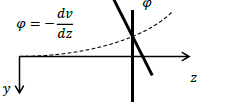
\includegraphics[width=0.5\linewidth]{figures/screenshot004}
				 	\label{fig:screenshot004.1}
				 \end{figure}
				 Vuol dire che se si avesse un contatto al di fuori di questo punto E si avrebbe interferenza.
				 
				 Il punto E mette in relazione la fondamentale della ruota con la retta di riferimento della dentiera.
				 
				 Il segmento CH cioè la distanza della retta di riferimento della dentiera dalla punta della dentiera è pari dunque a EC - segmento dei contatti utile massimo - per seno di tenta, ovvero 
				 \[CH = EC\sin\theta = R\sin^2\theta = \left(\dfrac{zm_0}{2}\right)\sin^2\theta\]
				 La condizione di non interferenza si verifica quando E può diventare un punto di contatto e quindi non appena lo  spostamento della primitiva diviene al più tale da portare la testa della dentiera nella posizione E, ovvero se e solo se si ha un raggio di primitiva  che risponda a questa relazione 
				 \[xm_0 = m_0 - \left(\dfrac{zm_0}{2}\right)\sin^2\theta\]
				 In caso di non correzione si aveva $z_0 = {2\over\sin^2\theta}$, si individua così, nel caso di correzione Lasche, che la condizione limite di interferenza, è data da 
				 \[x = 1 - \dfrac{z}{z_0}\]
				 Con $z$ numero di denti effettivamente realizzati e $z_0$ è il numero di denti limite in condizione di non correzione. \newline 
				 
				 Questo vuol dire che non si può andare al di sotto di tale valore di $x$, pena interferenza in fase di taglio. \newline 
				 
				 Il numero di denti viene notevolmente ridotto grazie alla correzione ed è estremamente importate per determinare un ottimo fattore di ricoprimento. 
				 
				 Il diagramma successivo dà un'idea dell'influenza del numero di denti di ruota e pignone, in funzione del fattore di ricoprimento. 
				 \begin{figure}[H]
				 	\centering
				 	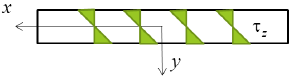
\includegraphics[width=0.5\linewidth]{figures/screenshot007}
				 	\label{fig:screenshot007}
				 \end{figure}
				 Se si vogliono alti fattori di ricoprimento si deve guardare in alto a destra, mentre i fattori di ricoprimento limite - unitari - sono rappresentatati dell'ultima curva in baso a sinistra. 
				 
				 Al tempo stesso però il numero di denti dev'essere contenuto: ridurre il numero di denti va sempre in contrasto con l'avere alti fattori di ricoprimento ed aumenta il rischio di interferenza. \newline 
				 
				 Il problema è che la correzione Lasche permette sì una riduzione dell'interasse, un miglioramento degli ingombri e della resistenza del dente del pignone, indebolendo però quello della ruota, ma non risponde all'esigenza del bilanciamento degli strisciamenti specifici, di conseguenza nella stragrande maggioranza dei casi, si utilizzano due coefficienti $x\ne x'$ che dovranno sempre rispettare la condizione limite di non interferenza di taglio come descritto in precedenza. \newline
				 
				 \textbf{NB:} notare che ogni volta che si sceglie un numero di denti superiore al minimo di non interferenza teorico, la quantità 
				 \[x = 1 - \dfrac{z}{z_0}<0\]
				 E quindi le correzioni positive sono sempre ammesse. 
				 
				 Se ci si spinge invece poco al di sotto di quello teorico, quindi con $z<z_0$, ad esempio scegliendo il numero di denti pratico secondo normativa DIN, allora 
				 \[x = 1 - \dfrac{z}{z_0}>0\]
				 E quindi non possono essere scelti valori anche di poco positivi. 
				 
				\end{adjustwidth}
\newpage
				\section{Correzioni diverse}
				\begin{adjustwidth}{2in}{}	
				Cosa succede se si scelgono correzioni diverse? 
				
				Si individuano due spessori sulla primitiva del tutto indipendenti l'uno dall'altro, con la conseguenza che la loro somma non fa più il passo. 
				
				Perciò se si forzano nella posizione originale, possono manifestarsi due casistiche 
				\begin{itemize}
					\item Compenetrazione, se la somma dei due spessori fornisce un risultato maggiore del passo.
					\item Scampanatura, se la somma dei due spessori fornisce un risultato minore del passo. 
					
					In questo caso il dente è più piccolo del vano non garantendo più continuità del moto.
				\end{itemize}
				Per evitare tali problematiche \textbf{le primitive di taglio non possono essere più usate come primitive di lavoro}, tuttavia i profili rimangono coniugati e ad evolvente, qual è allora come si può allora garantire il funzionamento? Si spostano o si avvicinano i centri di rotazione delle ruote; in questo modo cambiano soltanto le circonferenze primitive di lavoro, e quindi le grandezze cinematiche:  si sta cambiano il cinematismo. 
				
				Tra le conseguenze immediate si registra in output uno spostamento delle circonferenze che dipende da $x, x'$, poiché $x\ne x'$ è cambiata la proporzione tra le primitive e quindi cambierà il rapporto di trasmissione, l'interasse, la circonferenza primitiva di lavoro (che si realizza non appena si accoppiano due ingranaggi), la circonferenza di base e di testa, non cambierà la circonferenza fondamentale mentre la circonferenza primitiva di taglio sarà la semplice conseguenza dell'accoppiamento di taglio. \newline 
				
				Due ingranaggi corretti possiedono intrinsecamente delle circonferenze fondamentali fissate ed invariabili, nel momento in cui si accoppiano si individua il centro di istantanea rotazione e le circonferenze primitive di lavoro. 
				
				Chi mette in relazione le primitive di lavoro con le fondamentali? La retta tangente alle fondamentali che passa per il punto di istantanea rotazione (punto di tangenza delle primitive di LAVORO) 
				
				\begin{figure} [H]
					\centering
					\begin{tikzpicture}[scale=0.75]
					%%%	Help Lines
%					\draw [thin, help lines] (0,0) grid (10,10);
%					\foreach \x in {0,...,10}
%					\draw (\x cm,1pt) -- (\x cm,-1pt) node[anchor=north] {$\x$};
%					\foreach \y in {0,...,10}
%					\draw (1pt,\y cm) -- (-1pt,\y cm) node[anchor=east] {$\y$};
					
					%%% Punti
					\tkzDefPoints{8/6/omega1, 5/4/P, 5/10/C1, 5/1/C, 5/5/R1, 5/3.5/R}		
					\node [right] at (P) {$P$};		% Punto di contatto
					\node [right] at (C1) {$C'$}; 	% Centro condotta
					\node [right] at (C) {$C$};		% Centro motrice
					
					%%%	Disegno	
					\draw[thick, green] (10,10) arc (0:-180:5);
					\draw[thick, green] (2.5,1) arc (180:0:2.5);
					\draw[thick, red] (2,1) arc (180:0:3);
					\draw[thick, red] (11,10) arc (0:-180:6);
					%	\tkzDrawCircles(C1,R1 C,R)
					
					
					%%% Calcolo dei punti di tangenza
					\tkzDefTangent[from = P](C1,R1) \tkzGetPoints{T1a}{T1b}
					\tkzDefTangent[from = P](C,R) \tkzGetPoints{T2a}{T2b}
					% Questo comando calcola i punti di tangenza tra la circonferenza C1 e una retta passante per il punto P. I punti di tangenza vengono memorizzati in T1a e T1b.
					
					%%% Disegno della tangente
					\draw[thick] (P) -- ($(P)!1.5!(T1b)$) node[right] {$\Omega'$};
					\draw[thick] (P) -- ($(P)!1.5!(T2b)$) node[left] {$\Omega$};
					% Questo comando disegna la tangente dalla posizione di P al punto di tangenza % T1a sulla circonferenza C1. La parte ($(P)!1.5!(T1a)$) calcola un punto lungo la retta da P a T1a a una distanza del 150% dalla lunghezza della 
					% retta.
					\tkzDrawPoints (T1b,T2b,P, C, C1)
				\end{tikzpicture}
				\end{figure}
				\newpage
				Rispetto all'angolo d'attacco della dentiera $\theta_0$ che aveva  messo in relazione le primitive di taglio con la fondamentale, ora l'angolo è cambiato. 
				
				\begin{figure} [H]
					\centering
					\begin{tikzpicture}[scale=0.75]
					%%%	Help Lines
%					\draw [thin, help lines] (0,0) grid (10,10);
%					\foreach \x in {0,...,10}
%					\draw (\x cm,1pt) -- (\x cm,-1pt) node[anchor=north] {$\x$};
%					\foreach \y in {0,...,10}
%					\draw (1pt,\y cm) -- (-1pt,\y cm) node[anchor=east] {$\y$};
					
					%%% Punti
					\tkzDefPoints{8/6/omega1, 5/4/P, 5/10/C1, 5/1/C, 5/5/R1, 5/3.5/R}		
					\node [right] at (P) {$P$};		% Punto di contatto
					\node [right] at (C1) {$C'$}; 	% Centro condotta
					\node [right] at (C) {$C$};		% Centro motrice
					
					%%%	Disegno	
					\draw[thick, green] (10,10) arc (0:-180:5);
					\draw[thick, green] (2.5,1) arc (180:0:2.5);
					\draw[thick, red] (2,1) arc (180:0:3);
					\draw[thick, red] (11,10) arc (0:-180:6);
					%	\tkzDrawCircles(C1,R1 C,R)
					
					
					%%% Calcolo dei punti di tangenza
					\tkzDefTangent[from = P](C1,R1) \tkzGetPoints{T1a}{T1b}
					\tkzDefTangent[from = P](C,R) \tkzGetPoints{T2a}{T2b}
					% Questo comando calcola i punti di tangenza tra la circonferenza C1 e una retta passante per il punto P. I punti di tangenza vengono memorizzati in T1a e T1b.
					
					%%% Disegno della tangente
					\draw[thick] (P) -- ($(P)!1.5!(T1b)$) node[right] {$\Omega'$};
					\draw[thick] (P) -- ($(P)!1.5!(T2b)$) node[left] {$\Omega$};
					% Questo comando disegna la tangente dalla posizione di P al punto di tangenza % T1a sulla circonferenza C1. La parte ($(P)!1.5!(T1a)$) calcola un punto lungo la retta da P a T1a a una distanza del 150% dalla lunghezza della 
					% retta.
					\tkzDrawPoints (T1b,T2b,P, C, C1)
					
					\draw[thick] (0,4) -- (10,4);
					\draw[thick, <->] (6,4) arc (0:32:1) node [pos = 0.5, right] {$\theta$};
				\end{tikzpicture}
				\end{figure}
				
				L'angolo di pressione è diverso dell'angolo di attacco della dentiera. 
				 \[\theta\ne\theta_0\]
				Sono stati spostati i centri, la retta d'azione è stata ruotato. \newline 
				\end{adjustwidth}
				%\newpage
				\subsection{Grandezze corrette}
				\begin{adjustwidth}{2in}{}	
				\begin{itemize}
				\item In fase di correzione le 					\item $\theta = \theta_0 \Rightarrow R_0 = R$ - assenza di correzione   non cambiano.
				\[\rho = R_0\cos\theta_0 \qquad \rho' = R'_0\cos\theta_0\]
				Con $R_0$ raggio della circonferenza primitiva di taglio. 
				
				Con l'acquisto della ruota si ricevono delle informazioni anche sulla dentiera di realizzazione: dati $m_0, \theta_0$, quella dentiera messa ad una distanza $R_0$ (primitiva di taglio) dal centro della ruota, di ottiene come conseguenza geometrica, una circonferenza fondamentale $\rho$. \newline 
				
				\item La fondamentale durante il funzionamento non cambia, quindi il raggio di \textbf{primitiva di lavoro} sarà 
				\[R = \dfrac{\rho}{\cos\theta} = R_0\dfrac{\cos\theta_0}{\cos\theta} \qquad R = \dfrac{\rho'}{\cos\theta} = R'_0\dfrac{\cos\theta_0}{\cos\theta}\]
				Per cui, se
				\begin{itemize}
					\item $\theta = \theta_0 \Rightarrow R_0 = R$ - assenza di correzione  																												         \item $\theta \ne \theta_0 \Rightarrow R_0 \ne R$ - presenza di correzione  
				\end{itemize}
				
				\item Il \textbf{modulo} si era poi scritto come $m = D/z $ con $D$ diametro di primitiva. 
				
				Se cambia il diametro di primitiva allora anche il modulo sarà variato e quindi il modulo di lavoro (proprio ora della ruota dentata) sarà adesso pari, a causa della proporzione sui raggi primitivi, alla quantità 
				\[m = m_0\dfrac{\cos\theta_0}{\cos\theta}\] 
				
				\item L'\textbf{interasse}, ciò la somma dei due raggi di primitiva risulterà pari a 
				\[I = R+R'=\dfrac{m}{2}(z+z)\]
				La correzione introduce una variazione di interasse in funzione della variazione di modulo.
				\end{itemize}
%\newpage
				Nell'immagine seguente si possono individuare tutte le grandezze finora descritte.
				\begin{figure}[H]
					\centering
					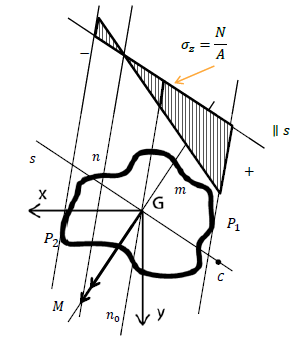
\includegraphics[width=0.5\linewidth]{figures/screenshot008}
					\label{fig:screenshot008}
				\end{figure}
				
				\textbf{NB:} ricorda che solo le primitive di funzionamento sono tangenti in $C$!\newline
				
				L'accoppiamento riportato in questa immagina è della tipologia in cui parte del profilo del dente NON segue l'evolvente, cioè tutta la dimensione radiale della circonferenza di piede e fondo, è tutto raccordo o parte rettilinea del dente, questo tuttavia comporta un vantaggio perché l'ultimo contatto utile avviene prima della circonferenza di base. \newline 
				
				\begin{itemize}
				\item Si immagini ora di rimuovere la condizione di gioco circonferenziale: la \textbf{condizione di corretto ingranamento} prevede (repetita iuvant) che la somma degli spessori sulle primitive di lavoro sia pari al passo, misurato sempre sulla circonferenza di lavoro, per cui:
				\[s + s' = \pi m\]
				Gli spessori sulle primitive di lavoro, per definizione di evolvente, si possono individuare a partire dalla relazione vista un paio di lezioni addietro:
				\[s = 2R(\ev\gamma - \ev\theta) = zm(\ev\gamma - \ev\theta) \qquad s' = 2R'(\ev\gamma' - \ev\theta) = z'm(\ev\gamma' - \ev\theta)\]
				Per cui
				\[s + s' = zm\ev\gamma + z'm\ev\gamma' - (z+z')m\ev\theta = \pi m\]
				Dove l'angolo $\theta$ è la variabile dell'evolvente, poiché si sia parlando del particolare raggio di primitiva $R$, questo è esattamente pari all'angolo di lavoro mentre $\ev\gamma$ ed $\ev\gamma'$ sono praticamente le semi-ampiezze angolari dei denti, ovvero gli angoli formati dai vertici dei prolungamenti dei profili dei denti del pignone e della ruota rispetto alle rette origine dell'evolvente, che sono da ricavare.  \newline				
				
				Gli angoli suddetti si possono ricavare a partire dagli spessori noti, ovvero sulla circonferenza primitiva di taglio, questa infatti è caratterizzata dalle seguenti dimensioni:
				\[R_0 = \dfrac{zm_0}{2} \qquad R_0' = \dfrac{z'm_0}{2}\] 
				\begin{itemize}
				\item Presenteranno uno \textbf{spessore del dente dal valore noto}, come inizialmente visto per le correzioni Lasche
				\[\begin{dcases}
					s_0 = \dfrac{\pi m_0}{2} + 2xm_0\tan\theta_0 = 2R_0(\ev\gamma - \ev\theta_0) \\
					s_0' = \dfrac{\pi m_0}{2} + 2x'm_0\tan\theta_0	= 2R_0'(\ev\gamma' - \ev\theta_0)				
				\end{dcases}\]
				\item Da queste relazioni si possono così ricavare le $\ev\gamma$
				\[\begin{dcases}
					\ev\gamma = \ev\theta_0 + \dfrac{2}{z}\left(\dfrac{\pi}{4} + x\tan\theta_0\right) \\
					\ev\gamma' = \ev\theta_0 + \dfrac{2}{z'}\left(\dfrac{\pi}{4} + x'\tan\theta_0\right) \\
				\end{dcases}\]
				\item Queste relazioni, sostituite nella formulazione della somma degli spessori, conducono a 
				\[\ev\theta = \ev\theta_0 + t\tan\theta_0 \dfrac{x+x'}{z + z'}\]
				Questa relazione permette di individuare la variazione dell'angolo di pressione in funzione del numero di denti e delle correzioni scelte. 
				
				Al fine poi di individuare l'angolo di lavoro $\theta$, si dovrà risolvere numericamente l'equazione della definizione di evolvente.
				\end{itemize} 
				
				\item Il \textbf{dedendum di taglio}, ovvero la sporgenza del dente della ruota rispetto alla circonferenza primitiva di taglio, ed è di relativamente facile individuazione:
				\[u = (1,25 - x)m_0 \qquad u' = (1,25 - x')m_0\] 
				Se la dentiera è stata spostata di una quantità pari ad $xm_0$, positivamente si è venuto a creare un minore scavo sulla base del dente, si è spostata la retta verso la punta della dentiera: la parte sporgente rispetto alla primitiva di taglio si è ridotto, e quindi si è ridotto anche lo scavo nella ruota dentata. 
				
				\item Tra le primitive di lavoro e di taglio vi è una \textbf{distanza radiale} definibile come grandezza differenza
				\[\begin{dcases}
					y = R-R_0 = \dfrac{z(m-m_0)}{2} = z \left(\dfrac{\cos\theta_0}{\cos\theta} - 1\right) m_0 = \eta m_0 \\										
					y' = R'-R'_0 = \dfrac{z'(m-m_0)}{2} = z' \left(\dfrac{\cos\theta_0}{\cos\theta} - 1\right) m_0 = \eta' m_0
				\end{dcases}\]
				La variazione di primitiva è così quantificabile attraverso queste relazioni. 
%\newpage				
				\item La variazione di \textbf{interasse}, cioè la differenza tra $(R-R') - (R_0-R_0')$ sarà quantificabile attraverso le grandezze $y$ appena definite come 
				\[\Delta I = y + y' = (\eta + \eta')m_0 = \xi m_0\]				
				\end{itemize}
				\vspace{0.5cm}
				
				Come cambiano ore le sporgenze del dente? 
				
				Tali sporgenze non varieranno perché frutto di moduli unificati, varieranno tuttavia i riferimenti dalle quali verranno misurate, questo è sempre alto ${9\over4}m_0$. 
				
				Quale si possono quantificare le sporgenze del dente rispetto alla primitiva di lavoro?
				\begin{itemize}
					\item \textbf{Dedendum di lavoro} \\
					Sapendo il dente rientrava di una quantità $u = (1,25 - x)m_0$, nel  momento in cui si sposta il riferimento di una quantità $\eta$, questa rientranza varierà proprio della quantità $\eta$. 
					\[u = (1,25 - x+\eta)m_0 \qquad u' = (1,25 - x'+\eta')m_0\]
					Quanto cambia la sporgenza del dente in fase di lavoro dipende da $x$, ovvero da una grandezza relativa al pignone, e da $\eta$ che non è una grandezza relativa al solo pignone, questa infatti dipende da $\cos\theta$, che a sua volta dipende da $x, x', z, z'$. 
					
					\item \textbf{Addendum Auspicato}\\
					È si cambiata la rientranza del dente, ma al tempo stesso si devono avere degli addendum che rispettino il gioco radiale: si è sicuri di non aver spinto in contatto radiale testa-piede? Perché d'altro canto gli $x, x'$ sono stati scelti in maniera indipendente. 
					
					Quanto dovrebbe essere allora l'addendum delle ruote? 
					\[a = u'- 0,25m_0 = (1-x'+\eta')m_0 \qquad a' = u- 0,25m_0 = (1-x+\eta)m_0\]
					Addendum del pignone dipende dal dedendum della ruota e viceversa. 
					
					Questi sono gli addendum auspicati, teorizzati, i minimi addendum che si devono avere per garantire gioco radiale. \newline
					
					Tuttavia con la correzione si è dovuto spostare tutto, è possibile quindi che questa dimensione venga violata, quali sono allora gli addendum effettivi di ruota e pignone? 
					
					\item \textbf{Addendum effettivi}\\
					L'addendum del pignone è la differenza tra l'altezza del dente ed il dedendum del dente, similmente per la ruota \[\begin{dcases}
						\bar{a} = \dfrac{9}{4}m_0 - \left(\dfrac{5}{4} -x + \eta\right)m_0 = (1+x-\eta)m_0 \\
						\bar{a}' = \dfrac{9}{4}m_0 - \left(\dfrac{5}{4} -x' + \eta' \right)m_0 = (1+x'-\eta')m_0
					\end{dcases}  \]
					Si può così osservare che l'addendum auspicato del pignone dipende da quanto è stata corretta la ruota, mentre l'addendum effettivo del pignone dipende da quanto è  stato corretto il pignone e similmente vale per la ruota: sono valori indipendenti tra loro. 
					
					Se confrontando questi due valori si trova che 
					\[\bar{a}<a\]
					Allora non si manifesta interferenza di piede, l'unica conseguenza sarà quella di avere un po' più di gioco radiale, il che non crea problemi. 
					
					Se invece 
					\[\bar{a}>a\]
					Si possono manifestare due conseguenze:
					\begin{enumerate}
						\item O una riduzione del gioco radiale: non ammessa.
						\item O un'interferenza sulla radice del dente: non ammessa.
					\end{enumerate}
					Come superare questa problematica? 
					
					Si utilizzerà in fase di realizzazione un rocchetto più piccolo: si manderà in lavorazione un rocchetto ridotto della  quantità pari alla differenza tra ciò che sarebbe effettivo e quello auspicato:
					\[\Delta = \bar{a}' - a' = \bar{a} - a = [(x+x') - (\eta+\eta')]m_0 = [(x+x')-\xi]m_0 = km_0\]
					Questa scelta si porta dietro un gioco radiale esattamente pari a quello auspicato, pari a $0,25m_0$; tuttavia si avrà un dente più basso di ${9\over4}m_0$, con conseguente riduzione del segmento dei contatti. \newline
					
					\textbf{NB:} Questa verifica comporta una riduzione del segmento dei contatti, si abbassa la troncatura esterna della ruota, è stata ridotta radialmente. 
					
					\item \textbf{Fattore di ricoprimento}\\
					Il fattore di ricoprimento è calcolabile in due modi:
					\begin{enumerate}
					\item O utilizzando la formula individuata nelle lezioni addietro, facendo attenzione ad utilizzare i corretti $k, k'$ ovvero le sporgenze delle ruote dentate rispetto alla circonferenza primitiva di lavoro, e quindi, nel caso specifico
					\[k = (1-x'+\eta')\dfrac{\cos\theta}{\cos\theta_0} \qquad k' = (1-x+\eta)\dfrac{\cos\theta}{\cos\theta_0}\]
					\item O attraverso la classica formula 
					\[\dfrac{\overline{AA'}}{p\cos\theta}\]
					\end{enumerate}
					\begin{figure}[H]
						\centering
						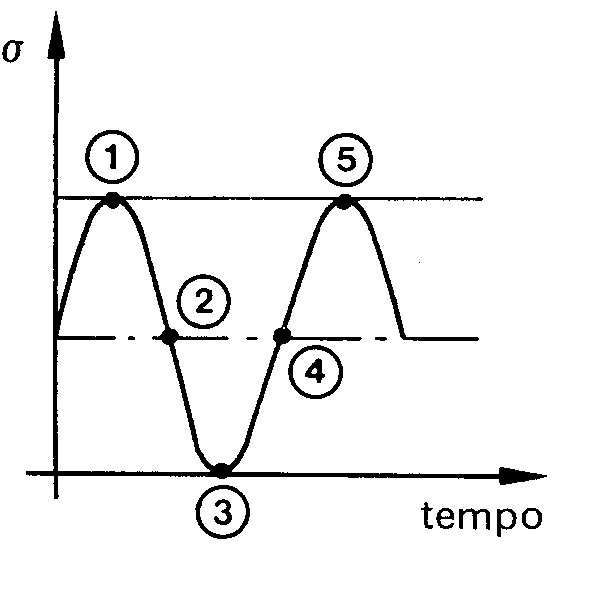
\includegraphics[width=0.3\linewidth]{figures/screenshot009}
						\label{fig:screenshot009}
					\end{figure}
					
					Se poi si fosse adoperata una riduzione della base del dente attraverso un'interferenza di taglio, si sarebbe ridotto, oltre al segmento teorico, anche quello effettivo dei contatti; questo perché riducendo il teorico, ci si sposta da T ad A, tagliando quella parte di evolvente dalla da $\rho\varphi$ e la circonferenza che passa per l'ultimo punto utile è quella per A, riducendo i potenziali punti di contatti dell'evolvente. 
					
					Ora se le troncature esterne di ruota e pignone cascano all'interno di quel segmento AA' il segmento effettivo dei contatti non ne risente, se invece la troncatura esterna fosse passata oltre gli ultimi punti A, il segmento dei contatti effettivo si sarebbe ridotto: fisicamente la testa della ruota si aspettava di trovare l'evolvente dell'altra, ma quel pezzo è stato rimosso e quindi non tocca nulla, il contatto è finito prima. 
					
					\item \textbf{Spessore in testa}\\
					Si dovrà sempre controllare lo spessore in testa del dente e si può fare attraverso le formulazioni già viste in precedenza
					\[s_t = 2r(\ev\gamma-\ev\theta_t)\geq0.2m_0\]
					Attenzione che il $\theta$ all'interno di questa formula NON è l'angolo di pressione, è la coordinata dell'evolvente, è  il $\theta_t$ corrispondente alla testa del dente, frutto della sua costruzione geometrica. 
					
					\item \textbf{Raggio di testa e di piede (di taglio o di lavoro)}\\
					Il raggio di testa sarà banalmente il raggio di primitiva sommato all'addendum e quello di piede vedrà il raggio di primitiva sottratto del dedendum. 
				\end{itemize}
\end{adjustwidth}
%\newpage
\subsection{Corretto funzionamento}
\begin{adjustwidth}{2in}{}	
	La condizione di ingranamento imposta, cioè che la somma degli spessori è al massimo uguale al passo è una condizione in realtà non realizzabile perché un piccolo gioco circonferenziale tra i denti è sempre necessario al fine di evitare che questi tocchino il profilo ozioso del dente successivo e per garantire il corretto film di lubrificazione dell'ingranaggio. \newline 
	
	Un piccolo gioco circonferenziale porta ad un leggero ingrandimento delle primitive e quindi una leggera variazione dell'interasse. 
	
	Il gioco necessario è molto piccolo: $\Delta s = \dfrac{1\div5}{100}m_0$, tuttavia questi valori portano ad un $\Delta I$ da dover considerare. \newline 
	
	La variazione di spessore $\Delta s$ che si deve garantire si può scrivere come la variazione della proiezione dei raggi di primitiva
	\[\Delta s = 2(\Delta R - \Delta R')\sin\theta = 2\Delta I\sin\theta\]
	Individuando una relazione che lega il gioco necessario alla variazione d'interasse. \newline 
	
	Nella pratica progettuale, se si ha la possibilità di variare l'interasse non sussiste alcun problema, in molte applicazioni però (automotive) l'interasse è fissato e non modificabile, in questo caso si effettueranno dei calcoli valutando un'interasse di riferimento 
	\[I_{rif} = I_{fissato} - \Delta I\] 
	Si dimensiona tutto il cinematismo con questo $I_{rif}$ e poi si individuerà il $I$ fissato dal problema.
	\[I_{rif} = \dfrac{1}{2}\dfrac{\cos\theta_0}{\cos\theta}(x+x')m_0\]
	In quest'ultima relazione è tutto noto; è possibile perciò ricavare $\cos\theta$, quindi $\theta$ e così ricavare i coefficienti di correzione da applicare alla ruote ad interasse fissato $(x + x')$. 
	
	Le correzioni $x$ ed $x$’ ottenute coi vari criteri prima detti, devono quindi essere ritoccate opportunamente in modo che la loro somma abbia il valore calcolato. Se il valore di $\theta$ risultasse molto diverso da quello assunto per il calcolo di $\Delta I$, i calcoli dovranno essere ripetuti fino a convergenza.
\end{adjustwidth}
%\newpage
\subsection{Scelta dei valori di correzione}
\begin{adjustwidth}{2in}{}	
	Con la correzione si può: 
	\begin{itemize}
		\item Irrobustire il dente
		\item Migliorare il fattore di ricoprimento 
		\item Bilanciare gli strisciamenti specifici
	\end{itemize}
	Il problema è che tutte queste dipendenze sono intrecciate e complesse, per cui non c'è una formulazione  univoca che definisca quali coefficienti $x, x'$ utilizzare. \newline
	
	Si deve perciò tenere conto a questo punto dei trend di comportamento.	
	\begin{itemize}
		\item Con $x+x'>0$ si ottiene un irrobustimento del dente ma un ridimensionamento del segmento di contatti. 
		\item Con $x+x'<0$ si ottiene una riduzione di interasse ed un aumento del fattore di ricoprimento 
	\end{itemize} 	
	\begin{figure}[H]
		\centering
		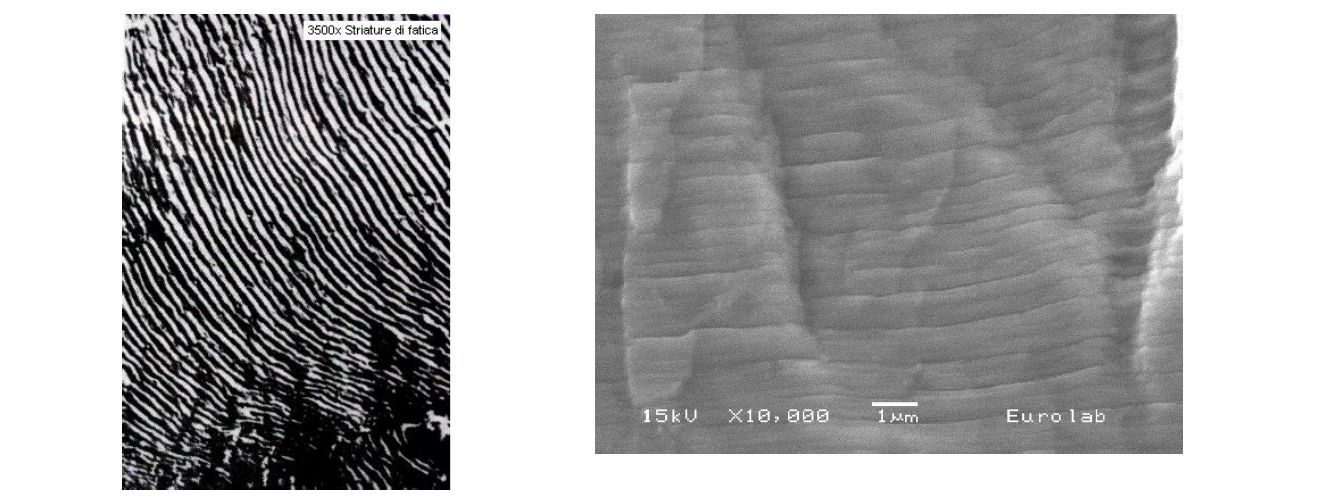
\includegraphics[width=0.3\linewidth]{figures/screenshot010}
		\label{fig:screenshot010}
	\end{figure}
	Le dipendenze sono perciò complesse: come si scelgono i valori di correzione? \newline 
	
	Si utilizzano le carte di Niemann, le quali forniscono delle indicazioni sulla scelta dei fattori correttivi. 
	
	Sono dei diagrammi piuttosto datati che forniscono un buon procedimento di massima utilizzabile tuttalpiù come riferimento, come primo approccio. \newline 
	
	Le carte di Neimann sono sostanzialmente 3, una generale che fornisce i valori di riferimento della somma di $x, x'$; una carta relativa ai riduttori ed una relativa ai moltiplicatori per definire singolarmente gli $x, x'$.  
\newpage
Nel primo diagramma si trovano i valori in ascissa pari alla somma del numero di denti e dei valori  in ordinata pari alla somma delle correzioni. 

La dipendenza tra ascisse e ordinate è dettata da  delle fasce di comportamento delle ruote dentate. \newline

Se ci si muove nelle zone alte si riscontrano dei casi in cui lo spessore alla base è molto grande   e il dente è molto robusto, al tempo stesso però il fattore di ricoprimento piccolo: sono  somme di correzioni molto elevate e positive. \newline 

In basso invece si trovano i casi in cui il fattore di ricoprimento è molto grande e vengono associati ad un dente più debole. \newline 

Dove ci si muove? Dipende dell'applicazione. 

Un'applicazione standard potrebbe attestarsi tra la P3 e la P5.
\begin{figure}[H]
	\centering
	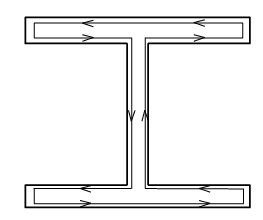
\includegraphics[width=0.7\linewidth]{figures/screenshot011}
	\label{fig:screenshot011}
\end{figure}
L'output è la somma delle correzioni. \newline 

A questo punto si entra nel diagramma dello specifico elemento (riduttore o moltiplicatore) 
\begin{figure}[H]
	\centering
	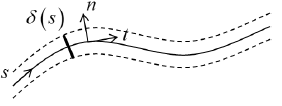
\includegraphics[width=0.7\linewidth]{figures/screenshot012}
	\caption{Riduttori}
	\label{fig:screenshot012}
\end{figure}
\begin{figure}[H]
	\centering
	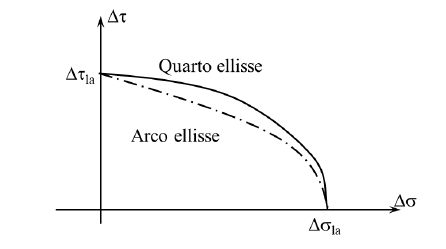
\includegraphics[width=0.7\linewidth]{figures/screenshot013}
	\caption{Moltiplicatori}
	\label{fig:screenshot013}
\end{figure}
E sempre tenendosi nelle fasce centrali delle classi di ingranaggi, si entra con la semisomma  del numero di denti in ascissa, ci si ferma all'altezza della  somma delle correzioni e si individua il punto $A$, a questo punto  si determina la retta che segua la tendenza  per interpolazione delle precedenti, ed entrando rispettivamente col numero di denti di ruota e pignone, si ottiene in output i valori di $x, x'$. \newline 

Questo metodo permette sì di migliorare le prestazioni ma non di individuare l'ottimo, nella pratica progettuale (progetto universitario proposto nel corso) si useranno in prima battuta le carte di Neimann, dopodiché ponendo come limite inferiore 
\[x = 1 - \dfrac{z}{z_0} \]
e ponendo il limite sulla somma pari a quello individuato dal Neimann, è possibile scrivere un codice iterativo che trovi l'ottimo tra i coefficienti di correzioni possibili che soddisfi tutte le verifiche richieste (spessore in testa, interferenza, fattore di ricoprimento, strisciamento), scegliendo il giusto criterio di scelta progettuale.
\end{adjustwidth}
\newpage
\section{Spinte sugli alberi}
\begin{adjustwidth}{2in}{}  
	Se $Q$ è pari alla spinta utile per creare momento torcente, ovvero quella periferica, allora la forza scambiata tra i denti sarà 
	\[N = \dfrac{Q}{\cos\theta}\]
	Inclinata di un angolo $\theta$ rispetto all'orizzontale. \newline 
	
	La componente di forza radiale, dalla trigonometria è individuabile come \[R = N\sin\theta = Q\tan\theta\]
	\begin{figure}[H]
		\centering
		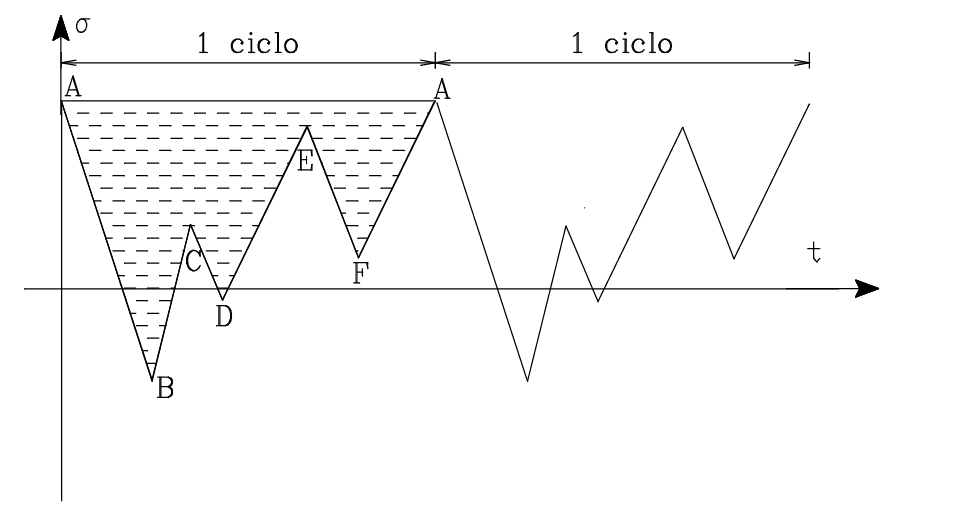
\includegraphics[width=0.5\linewidth]{figures/screenshot014}
		\label{fig:screenshot014}
	\end{figure}
	Per un albero motore da una sola ruota dentata le sole forze in gioco sono quelle ovviamente derivanti da quell'unica ruota dentata, se invece sono presenti più di una ruota dentata, come l'albero di rinvio in figura sopra, dove si possono individuare una ruota condotto ed una ruota motrice, allora le forze  in gioco saranno sia quelle relative alla condotto che quelle relative alla conduttrice.\newline 
	
	\textbf{NB:} il dimensionamento dell'albero deve tenere conto delle componenti circonferenziali e radiali che agiscono sui due piani ortogonali tra loro, per cui si avranno flessioni nel piano $xy$ e flessioni nel piano $xz$, ma anche i punti di ingranamento saranno importanti. 
	
	In questo caso dalla parte delle $z$ positive si avrà l'ingranamento della condotta, mentre a $180^\circ$ dall'alta parte, avverrà l'ingranamento del pignone dell'altro ingranaggio, per cui se si guarda l'albero concorde ad $x$, si vede sulla ruota condotta e conduttrice, delle forze applicate in punti diversi.
	
\begin{figure}[H]
	\centering
	\begin{tikzpicture}[>=latex, scale = 0.5]
%	%%%	Help Lines
%	\draw [thin, help lines] (0,0) grid (10,10);
%	\foreach \x in {0,...,10}
%	\draw (\x cm,1pt) -- (\x cm,-1pt) node[anchor=north] {$\x$};
%	\foreach \y in {0,...,10}
%	\draw (1pt,\y cm) -- (-1pt,\y cm) node[anchor=east] {$\y$};
	%%%	Disegno	
	\draw[thick, ->] (5,5) -- (11,5) node [pos = 1, right] {$z$};
	\draw[thick, ->] (5,5) -- (5,11) node [pos = 1, above] {$y$};
	\draw[ultra thick, red] (5,5) circle (2.5cm);
	\draw[ultra thick, blue] (5,5) circle (4cm);
		\draw [blue, ultra thick] (8.5, 5.5) -- (9.5,4.5);
	\draw [blue, ultra thick] (8.5, 4.5) -- (9.5,5.5);
	\draw [red, ultra thick] (2, 5.5) -- (3,4.5);
	\draw [red, ultra thick] (2, 4.5) -- (3,5.5);
\end{tikzpicture}
\end{figure}
	
	Quando si vanno a riportare sui piani $xy$ e $xz$ queste forze, creeranno flessione  secondo due piani diversi e si combineranno. 
	
	In questo caso le forze radiali e quelle circonferenziali giacciono nello stesso piano, ma se i punti di ingranamento fossero stati diversi, perché magari si decide di posizionare l'albero di rinvio a fianco di quello motore, ma magari poi si mette l'albero condotto di sopra:
	
\begin{figure}[H]
	\centering
	\begin{tikzpicture}[>=latex, scale = 0.5]
	%%%	Help Lines
%	\draw [thin, help lines] (0,0) grid (10,10);
%	\foreach \x in {0,...,10}
%	\draw (\x cm,1pt) -- (\x cm,-1pt) node[anchor=north] {$\x$};
%	\foreach \y in {0,...,10}
%	\draw (1pt,\y cm) -- (-1pt,\y cm) node[anchor=east] {$\y$};
	%%%	Disegno	
	\draw[thick, ->] (5,5) -- (11,5) node [pos = 1, right] {$z$};
	\draw[thick, ->] (5,5) -- (5,11) node [pos = 1, above] {$y$};
	\draw[ultra thick, red] (5,5) circle (2.5cm);
	\draw[ultra thick, blue] (5,5) circle (4cm);
	\draw [blue, ultra thick] (8.5, 5.5) -- (9.5,4.5);
	\draw [blue, ultra thick] (8.5, 4.5) -- (9.5,5.5);
	\draw [red, ultra thick] (2, 5.5) -- (3,4.5);
	\draw [red, ultra thick] (2, 4.5) -- (3,5.5);
	% Forze 
	\draw [->, blue, ultra thick] (9, 5) -- (7.5,5);
	\draw [->, blue, ultra thick] (9, 5) -- (9,1);
	\draw [->, red, ultra thick] (2.5, 5) -- (4,5);
	\draw [->, red, ultra thick] (2.5, 5) -- (2.5, 3);
\end{tikzpicture}
\end{figure}
	
	E allora nello stesso piano ci saranno le forze radiali di un ingranaggio e quelle circonferenziali dell'altro, e viceversa.  
	
	\textbf{ATTENZIONE AI PUNTI DI INGRANAMENTO, FANNO CAMBIARE COMPLETAMENTE IL DIMENSIONAMENTO DELL'ALBERO.} \newline 
	
	Come è possibile ricostruire il verso di rotazione dell'albero a partire dalla forze scambiate? (rispetto a x).
	
	(positivo antiorario, negativo orario) 
	
	Sulla ruota condotta la forza periferica è concorde con la rotazione, perché è una forza che la ruota subisce, sulla ruota  motrice è invece una forza di resistenza: sta ruotando e trova la resistenza dell'albero condotto e subisce per reazione quella forza. 
	
	Per cui sulla ruota motrice la forza periferica è contrapposta alla rotazione, mentre sulla ruota condotta la forza circonferenziale è orientata come la rotazione. \newline
	
	Nell'immagine sopra, la rotazione della condotta è positiva (verso del vettore in funzione della posizione di ingranamento), perché l'albero  ruota in direzione oraria.  \newline 
	
	Se si piazza la ruota dentata tra gli appoggi in schema appoggio - appoggio il momento flettente sarà massimo al centro e le reazioni vincolari sui cuscinetti saranno piuttosto piccole, se invece la ruota viene montata a sbalzo, il momento flettente massimo sarà sul cuscinetto, con relative reazioni vincolari molto più grandi. 
	
	\begin{figure}[H]
		\centering
		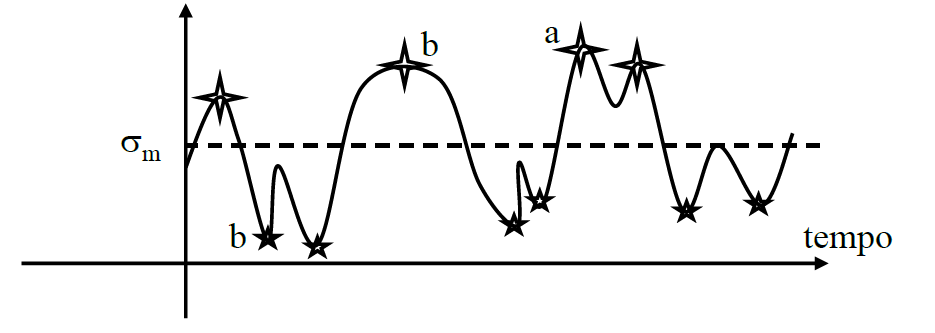
\includegraphics[width=0.8\linewidth]{figures/screenshot015}
		\caption{Alcuni schemi di montaggio}
		\label{fig:screenshot015}
	\end{figure}
		

	
	
	
	





	
	
	
	
				
				
				
				
							 
				  
				 
				 
				 
				
				
				
				
				
				
				
				
				
				
				
			
			
			
			
			
			
			
			
			
			
			
			
			
			
			
			
			
			
			
			
			
			
			
			
			
			
			
			
				
			\end{adjustwidth}	
		\end{document}
